% Standalone figure for CMR submission
% The Learning Velocity Framework
% Compile with: pdflatex figure1-framework.tex

\documentclass[tikz,border=10pt]{standalone}

\usepackage[T1]{fontenc}
\usepackage{lmodern}
\usetikzlibrary{shapes.geometric,arrows.meta,positioning,calc,decorations.pathreplacing}

\begin{document}

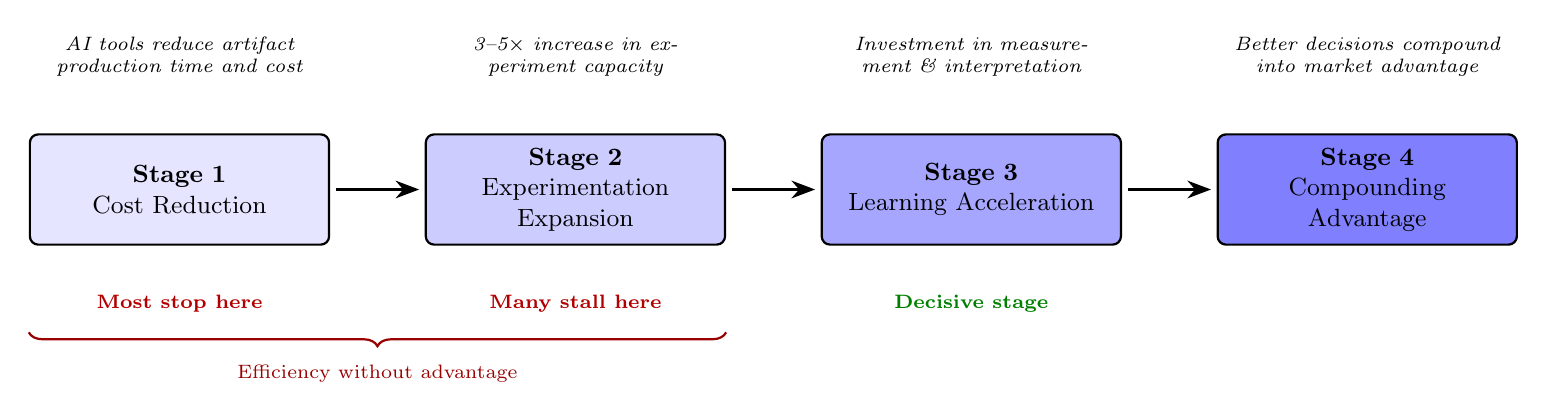
\begin{tikzpicture}[
    stage/.style={
        rectangle,
        rounded corners=3pt,
        draw=black,
        thick,
        minimum width=3.8cm,
        minimum height=1.4cm,
        text centered,
        text width=3.4cm,
        align=center,
        font=\small
    },
    arrow/.style={
        -{Stealth[length=3mm]},
        thick,
        shorten >=2pt,
        shorten <=2pt
    },
    annotation/.style={
        font=\scriptsize\itshape,
        text width=3.5cm,
        align=center
    },
    failpoint/.style={
        font=\scriptsize\bfseries,
        text=red!70!black
    }
]

% Stages
\node[stage, fill=blue!10] (s1) {
    \textbf{Stage 1}\\Cost Reduction
};

\node[stage, fill=blue!20, right=1.2cm of s1] (s2) {
    \textbf{Stage 2}\\Experimentation Expansion
};

\node[stage, fill=blue!35, right=1.2cm of s2] (s3) {
    \textbf{Stage 3}\\Learning Acceleration
};

\node[stage, fill=blue!50, right=1.2cm of s3] (s4) {
    \textbf{Stage 4}\\Compounding Advantage
};

% Arrows
\draw[arrow] (s1) -- (s2);
\draw[arrow] (s2) -- (s3);
\draw[arrow] (s3) -- (s4);

% Annotations above
\node[annotation, above=0.6cm of s1] {AI tools reduce artifact production time and cost};
\node[annotation, above=0.6cm of s2] {3--5$\times$ increase in experiment capacity};
\node[annotation, above=0.6cm of s3] {Investment in measurement \& interpretation};
\node[annotation, above=0.6cm of s4] {Better decisions compound into market advantage};

% Failure points below
\node[failpoint, below=0.5cm of s1] {Most stop here};
\node[failpoint, below=0.5cm of s2] {Many stall here};
\node[failpoint, below=0.5cm of s3, text=green!50!black] {\textbf{Decisive stage}};

% Bracket showing common failure zone
\draw[thick, red!60!black, decorate, decoration={brace, amplitude=5pt, mirror}]
    ([yshift=-1.1cm]s1.south west) -- ([yshift=-1.1cm]s2.south east)
    node[midway, below=8pt, font=\scriptsize, text=red!60!black] {Efficiency without advantage};

\end{tikzpicture}

\end{document}
